\documentclass[jou]{apa6}

\usepackage[american]{babel}

\usepackage{csquotes}
\usepackage[style=apa,sortcites=true,sorting=nyt,backend=biber]{biblatex}
\DeclareLanguageMapping{american}{american-apa}
\addbibresource{bibliography.bib}


%%%%%%%%%%%%%%%%%%%%%%%%%%%%%%%%%%%%%%%%
%% Discrete Structures
%% The start of RBS stuff
%%%%%%%%%%%%%%%%%%%%%%%%%%%%%%%%%%%%%%%%

% Working internal and external links in PDF
\usepackage{hyperref}
% Extra math symbols in LaTeX
\usepackage{amsmath}
\usepackage{gensymb}
\usepackage{amssymb}
% Enumerations with (a), (b), etc.
\usepackage{enumerate}

\let\OLDitemize\itemize
\renewcommand\itemize{\OLDitemize\addtolength{\itemsep}{-6pt}}

\usepackage{etoolbox}
\makeatletter
\preto{\@verbatim}{\topsep=3pt \partopsep=3pt }
\makeatother

% These sizes redefine APA for A4 paper size
\oddsidemargin 0.0in
\evensidemargin 0.0in
\textwidth 6.27in
\headheight 1.0in
\topmargin -24pt
\headheight 12pt
\headsep 12pt
\textheight 9.19in



\setlength\parindent{0pt}

\title{Midterm, 2020-02-17}
\author{Discrete Structures, Fall 2020}
\affiliation{RBS}

\leftheader{Midterm, 2020-02-17}

\abstract{%
}

%\keywords{}

\begin{document}

\thispagestyle{empty}

\twocolumn
{\Large Midterm, 2020-02-17}

\vspace{6pt}
{\bf Question 1 (Boolean Expressions).}\\
Consider Boolean expression:
$$E_0 = (p \rightarrow q \rightarrow r) \wedge (q \rightarrow r \rightarrow p) \wedge (r \rightarrow p \rightarrow q)$$
\begin{center}
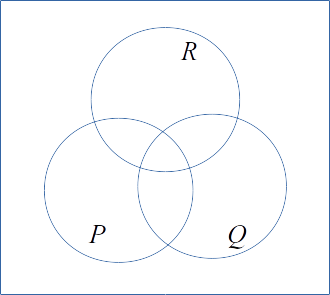
\includegraphics[width=2in]{midterm/circles.png}
\end{center}

\begin{enumerate}[(A)]
\item Copy the Venn diagram's circles in your solution and shade those regions in the diagram that make $E_0$ true
(being inside each circle $P,Q,R$ means that the respective variable $p,q,r$ is true; being outside the circle means
that the variable is false). 
\item In the truth table of $E_0$ how many entries are $\mathtt{True}$?\\
({\em Note.} Building the truth table is optional. Regardless whether you build one or not, you should justify your answer.)
\item Rewrite the Boolean expression $E_0$ into an equivalent one, using 
only conjunctions ($\wedge$) and negations ($\neg$). 
\end{enumerate}

Assume that implication ($\rightarrow$) is right-associative 
and conjunction ($\wedge$) has higher precedence than implication. 



\vspace{10pt}
{\bf Question 2 (Nested Quantifiers).}\\
Verify, if the following predicate/quantifier expressions are true for the given predicate. 
The predicate $P$ is defined on $A \times A$, where
$A = \{ \mathtt{a},\mathtt{b},\mathtt{c},\mathtt{d},\mathtt{e},\mathtt{f} \}$. 
Predicate $P(\mathtt{a},\mathtt{b})$ is true iff the square on row $\mathtt{a}$
and column $\mathtt{a}$ is shaded (and the predicate $P(\mathtt{a},\mathtt{b})$ 
is false, if that square is white).

\begin{center}
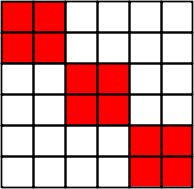
\includegraphics[width=1.2in]{midterm/relation.png}
\end{center}

\begin{enumerate}[(A)]
\item Does the predicate $P$ satisfy the logic formula:
$$\forall i \in A,\;P(i,i).$$
\item Does the predicate $P$ satisfy the logic formula:
$$\forall i \in A,\,\forall j \in A,\;P(i,j) \rightarrow P(j,i).$$
\item Does the predicate $P$ satisfy the logic formula:
$$\forall i,j,k \in A,\;P(i,j) \wedge P(j,k) \rightarrow P(i,k).$$
\item Does the predicate $P$ satisfy the logic formula:
$$\forall i,j \in A,\;P(i,j) \vee P(j,i).$$
\item Does the predicate $P$ satisfy the logic formula:
$$\forall i \in A,\, \exists j \in A,\;P(i,j).$$
\end{enumerate}

\vspace{10pt}
{\bf Question 3 (Estimate with Big-O Notation).}\\
Define the sequence $S(n)$ as a sum of squares from $1^2$ to $n^2$:
$$S(n) = \sum\limits_{i=1}^n i^2.$$
We have $S(1) = 1^2 = 1$, $S(2) = 1^2 + 2^2 = 5$, 
$S(3) = 1^2 + 2^2 + 3^2 = 14$,
and so on. 

\begin{enumerate}[(A)]
\item Is the function $S(n)$ in $O(n^1)$? 
Is it in $O(n^2)$? Is it in $O(n^3)$? Is it in $O(n^4)$? 
Explain your reasoning. 
\item Pick any one of the notations from the previous items 
($g(n)$ is either $O(n^1)$, or $O(n^2)$, or $O(n^3)$, or $O(n^4)$). 
Check the definition of Big-O notation: Find the {\em witness}: the value $k$ and the constant $C$
such that the absolute value of $S(n)$ does not exceed $C\cdot{}|g(n)|$ for all $n > k$.
\end{enumerate}


\vspace{10pt}
{\bf Question 4 (Chinese Remainder Theorem).}

Consider the following system of three congruences:
$$\left\{ \begin{array}{l}
x \equiv 1\;(\text{mod}\,5),\\
x \equiv 2\;(\text{mod}\,7),\\
x \equiv 3\;(\text{mod}\,9).
\end{array} \right.$$

\begin{enumerate}[(A)]
\item Does it have a solution? Will it have solution, even if we replace $1,2,3$ with other numbers
on the right sides of the equation.
\item Find an arithmetic progression (what is its first member $A$, difference $B$) where all members satisfy
the first two congruences from the system.
\item Find an arithmetic progression (what is its first member $C$, difference $D$) where all members satisfy
all three congruences in the system.
\end{enumerate}

{\em Note.} Arithmetic progression is an infinite sequence where every next member can be obtained
by adding the same number (the difference) to the previous one. For example, 
$$A,\;A+B,\;A+2B,\;A+3B,\ldots$$
is an arithmetic progression with the first member $A$ and the difference $B$.


\vspace{10pt}
{\bf Question 5 (Binary notation).}

Somebody has written two binary fractions on the board: $\alpha$ is infinite, $\beta$ is finite (just $6$ digits
after the point): 
$$\left\{ \begin{array}{l}
\alpha = 0.(011110)_2 = 0.011110011110011110\ldots_2\\
\beta = 0.011110_2.
\end{array} \right.$$

\begin{enumerate}[(A)]
\item Express the number $\beta$ as a sum of some negative powers of $2$; 
namely, show how to add up some of the numbers
$$\{ 2^{-1}, 2^{-2}, 2^{-3}, \ldots \}$$ 
to get $\beta$. 
\item Express $\beta$ as an irreducible fraction {\tt P/Q}; write this in the regular decimal notation. 
\item Write the product $64_{10} \cdot \alpha = 1000000_2 \cdot \alpha$ in the binary notation. 
\item Express $\alpha$ as an irreducible fraction {\tt P/Q} in decimal notation.
\end{enumerate}



\vspace{10pt}
{\bf Question 6 (Truth-tellers and Liars).}
Among the people $A,B,C$ one is a truth-teller, 
the other two are liars. 
Every person ($A$, $B$, and $C$) has a closed box
in front of himself/herself. Exactly one of the 
boxes has a candy inside. $A,B,C$ know everything 
about each other and the location of candy.

Someone else (person $D$) approaches all of them. $D$ knows, who are 
people $A$,$B$, and $C$ (it is written on their name-cards), but $D$ does
not know anything about their lying behavior or the location of the candy.
$D$ is allowed to ask YES/NO questions to one or more people.

\begin{enumerate}[(A)]
\item Can $D$ find out who has the candy by asking three questions?
\item Can $D$ find out who has the candy by asking two questions?
\item Can $D$ find out who has the candy by asking one question?
\end{enumerate}

Justify your answers (by construction or by showing that it is impossible).


\vspace{10pt}
{\bf Question 7 (Time Complexity of Truth Tables).}

Assume that there is a Boolean expression $E$ with $n$ variables: 
$$E = E(a_1,a_2,\ldots,a_n).$$
The expression $E$ contains $2n$ Boolean operators (such as $\neg$, $\wedge$, $\vee$).
Variables $a_1,a_2,\ldots,a_n$ can independently take values 
$\mathtt{True}$ or $\mathtt{False}$.

Consider the following algorithm to find, if $E$ is a tautology by 
building the truth table. We will either find a false value, or 
establish that all values were true (in this case $E$ is a tautology).

{\bf (1)} \hspace{0.0in} For each assignment of $n$ truth values to $a_1,\ldots,a_n$:\\
{\bf (2)} \hspace{0.2in} For each of the $2n$ Boolean operators in $E$:\\
{\bf (3)} \hspace{0.4in} Compute the value of that Boolean operator\\
{\bf (4)} \hspace{0.2in} If $E$ has value $\mathtt{False}$:\\
{\bf (5)} \hspace{0.4in} Return ``$E$ is not a tautology.''\\
{\bf (6)} \hspace{0.2in} If $E$ has value $\mathtt{True}$:\\
{\bf (7)} \hspace{0.4in} Continue loop on Line {\bf (1)}.\\
{\bf (8)} \hspace{0.0in} Return ``$E$ is a tautology.''

\begin{enumerate}[(A)]
\item Find the worst-case runtime $T(n)$ for this algorithm as an expression of $n$.
(Assume that evaluating one Boolean operator $\neg$, $\wedge$, $\vee$ takes $1$ unit of time.)
\item Find a function $g(n)$ such that $T(n)$ is in $O(g(n))$. 
\end{enumerate}




\vspace{10pt}
{\bf Question 8 (About Rational and Irrational).}

We denote two real numbers by $p$ and $q$. 
Prove or disprove statements about the rational and irrational numbers. 

\begin{enumerate}[(A)]
\item If $p + q$ is rational, then either both $p,q$ are rational, or both are irrational. 
\item If $pq$ is rational, then either both $p,q$ are rational, or both are irrational. 
\item If $p^2$ and $q^2$ are both rational, then the product $(p+q)(p-q)$ is rational. 
\item If $p^3$ and $p^5$ are both rational, then $p$ is rational.
\item If $pq$ and $p+q$ are both rational, then $p$ and $q$ are both rational.
\end{enumerate}


\end{document}

